% !TeX root = ./../main.tex

\subsection{Experiment A}

The resonance curve of the vibrating reed was measured around the first three harmonic frequencies.
\num{20} independent measurements of the amplitude/phase shift/$X$/$Y$ were taken at each frequency, then immediately averaged, with standard deviation taken to be the error.
These datasets were saved to text files for analysis.
In our analysis code we read in the data again.
The measurements are plotted against frequency and displayed in \autoref{fig:analysis_exp_a}.

\begin{figure}[htbp]
    \centering
    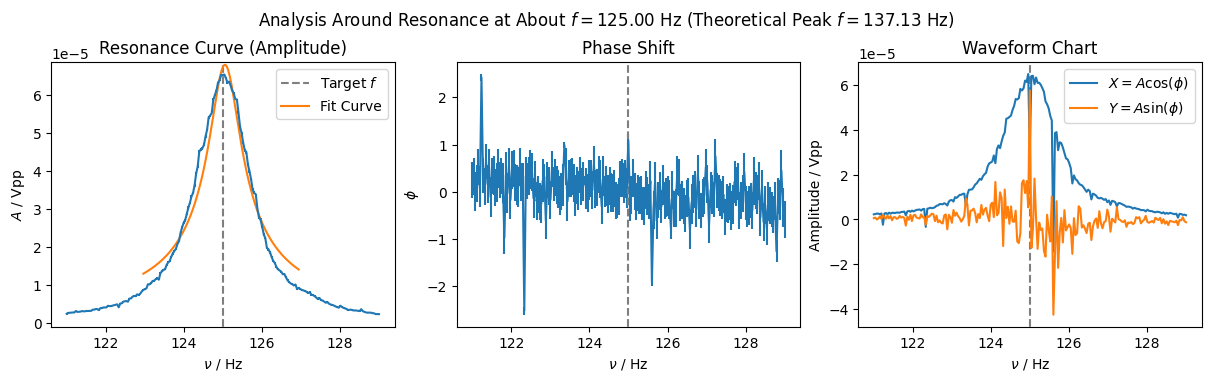
\includegraphics[width=0.85\textwidth]{res1.png}
    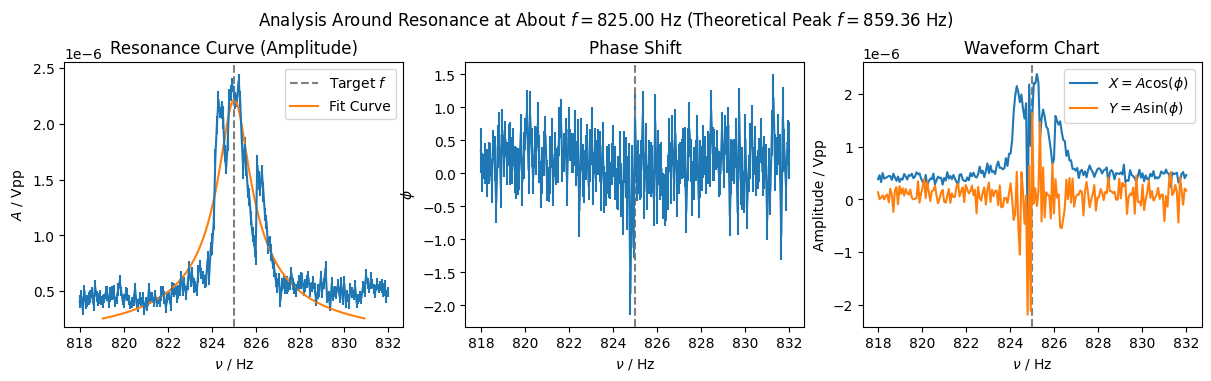
\includegraphics[width=0.85\textwidth]{res2.png}
    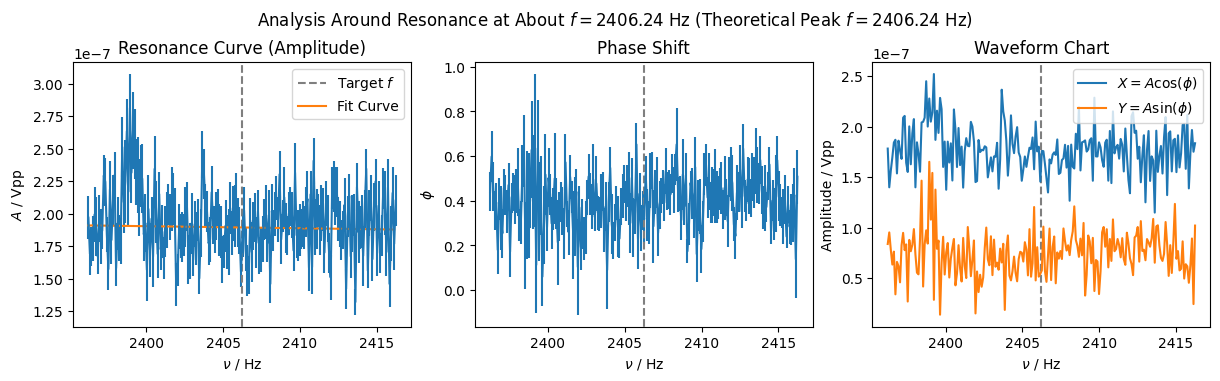
\includegraphics[width=0.85\textwidth]{res3.png}
    \caption{Resonance Curves at First Three Harmonics}
    \label{fig:analysis_exp_a}
\end{figure}

In the graphs we also plot the "target frequency" around which the peak is expected to be.
Lastly, we use regression (least squares/parametric $\chi^2$ fit) to fit a Lorentz curve (see \autoref{eq:analysis_lorentz}) to the resonance peak for each dataset.
The resulting parameters and fit statistics are given in \autoref{tab:analysis_params_a}

\begin{table}[htpb]
    \centering
    \caption{}
    \label{tab:analysis_params_a}
    \(\begin{tabular}{
        S[table-format=4.0]
        S
        S
        S
        S
        S
        S
        S
    }
        {$f_\mathrm{target}$} & {$f_0$} & {$\omega_0$}& $\gamma$ & {$\chi^2$} & {$\chi^2_\mathrm{red}$} & {$p$} & Q \\ \hline
        125  \\
        825  \\
        2406 
    \end{tabular}\)
\end{table}
